%% BEAMER THEME FLIP 2012: Main tex file for compiling
%$ Compile this file. 
%%
%% Copyright 2012 by Flip Tanedo
%% This file may be distributed and/or modified
%% 	1. under the LaTeX Project Public License and/or
%% 	2. under the GNU Public License.
%% 
%% If you e-mail Flip (pt267@cornell.edu) to say that you
%% like this style file, then it would make him smile.

%% Please see notes.txt for comments on Beamer Theme Flip 2013
%% By default, this template is meant to be run with XeLaTeX (for fonts)
%% To run in PDFLaTeX, remove fontspec and any font commands

%% Discussion of Beamer vs XeLaTeX vs LuaLaTeX
%% http://tex.stackexchange.com/questions/29497/xelatex-preventing-beamer-from-using-different-backgrounds



\documentclass[12 pt,xcolor={table}]{beamer}
\usetheme[
	bullet=circle,		% Other option: square
	bigpagenumber,		% circled page number on lower right
	topline=true,			% colored bar at the top of the frame 
	shadow=false,			% Shading for beamer blocks
	watermark=BG_lower,	% png file for the watermark
	]{Flip}


\newcommand{\titleimage}{title}			% Custom title 
\newcommand{\tanedo}{tanedolight}		% Custom author name
\newcommand{\CMSSMDM}{CMSSMDMlight.png}	% light background plot


%%%%%%%%%%
% FONTS %
%%%%%%%%%%

%% Default font: lmodern, doesn't require fontspec % solves some default warnings
\usepackage[T1]{fontenc}
\usepackage{lmodern}			
%\usepackage{sfmath}		% Sans Serif Math, off by default


%% Protects fonts from Beamer screwing with them
%% http://tex.stackexchange.com/questions/10488/force-computer-modern-in-math-mode
\usefonttheme{professionalfonts}


%% XeLaTeX fonts: (comment out if you don't use XeLaTeX)

%% For advanced fonts: access local OS X fonts
\usepackage[no-math]{fontspec}		
%% This template uses typical OS X and Adobe fonts
\defaultfontfeatures{Mapping=tex-text}	% This seems to be important for mapping glyphs properly

\setmainfont{Gillius ADF Regular} % Beamer ignores "main font" in favor of sans font
\setsansfont{Gillius ADF Regular}	% This is the font that beamer will use by default
% \setmainfont{Gill Sans Light}		% Prettier, but harder to read

\setbeamerfont{title}{family=\fontspec{Gillius ADF Regular}}


\newcommand{\handwriting}{\fontspec{augie}} % From Emerald City, free font
% \newcommand{\handwriting}{}	% If you prefer no special handwriting font or don't have augie

%% Gill Sans doesn't look very nice when boldfaced
%% This is a hack to use Helvetica instead
%% Usage: \textbf{\forbold some stuff}
\newcommand{\forbold}{\fontspec{Gillius ADF Cond Bold}}
% \newcommand{\forbold}{} % if you want no special boldface



%%%%%%%%%%%%%%%%%%%%%%%%
% Usual LaTeX Packages %
%%%%%%%%%%%%%%%%%%%%%%%%


\usepackage{amsmath}
\usepackage{amsfonts}
\usepackage{amssymb}
\usepackage{graphicx}
\usepackage{mathrsfs} 			% For Weinberg-esque letters
\usepackage{cancel}				% For "SUSY-breaking" symbol
\usepackage{slashed}            % for slashed characters in math mode
\usepackage{bbm}                % for \mathbbm{1} (unit matrix)
\usepackage{amsthm}				% For theorem environment
\usepackage{multirow}			% For multi row cells in table
\usepackage{arydshln} 			% For dashed lines in arrays and tables
\usepackage{tikzfeynman}		% For Feynman diagrams
% \usepackage{subfig}           % for sub figures
% \usepackage{young}			% For Young Tableaux
% \usepackage{xspace}			% For spacing after commands
% \usepackage{wrapfig}			% for Text wrap around figures
% \usepackage{framed}


\graphicspath{{img/}}	% Put all images in this directory. Avoids clutter.

\usetikzlibrary{arrows,shapes}
\usetikzlibrary{fadings}
\usetikzlibrary{backgrounds}
\usetikzlibrary{mindmap,trees}	% For mind map
% http://www.texample.net/tikz/examples/computer-science-mindmap/


% SOME COMMANDS THAT I FIND HANDY
% \renewcommand{\tilde}{\widetilde} % dinky tildes look silly, dosn't work with fontspec
\newcommand{\comment}[1]{\textcolor{comment}{\footnotesize{#1}\normalsize}} % comment mild
\newcommand{\Comment}[1]{\textcolor{Comment}{\footnotesize{#1}\normalsize}} % comment bold
\newcommand{\COMMENT}[1]{\textcolor{COMMENT}{\footnotesize{#1}\normalsize}} % comment crazy bold
\newcommand{\Alert}[1]{\textcolor{Alert}{#1}} % louder alert
\newcommand{\ALERT}[1]{\textcolor{ALERT}{#1}} % loudest alert
%% "\alert" is already a beamer pre-defined



\author[Mandy Vogel\quad {mandy.vogel@googlemail.com}]{Mandy Vogel}
\title[Models/Anova]{Models/Anova}
\institute{University Leipzig}
\date{\today}



\begin{document}

%%%%%%%%%%%%%%%%%%%%%%%%
% Additional  settings %
%%%%%%%%%%%%%%%%%%%%%%%%

%% To use external nodes;  http://www.texample.net/tikz/examples/beamer-arrows/
\tikzstyle{every picture}+=[remember picture]


\everymath{\displaystyle}

\tikzfading[name=fade inside,
            inner color=transparent!60,
            outer color=transparent!0]
%%%%%%%%%%%%%%%%%%%%%%%%
% Actual content below %
%%%%%%%%%%%%%%%%%%%%%%%%

%% It's much nicer to have all the content in a separate file


\AtBeginSection{
  \begin{frame}<beamer>[allowframebreaks,t]{Table of Contents}
    \tableofcontents[currentsection]
  \end{frame}}


\begin{frame}
\titlepage
\end{frame}

\begin{frame}{Overview}
  \tableofcontents
\end{frame}

\section{Combining Data Frames}
\subsection{\texttt{rbind()}}
\begin{frame}[fragile]\frametitle{\texttt{rbind()}}
\begin{itemize}
\item \texttt{rbind()} can be used to combine two dataframes (or matrices) in the sense of adding rows, the column names and types must be the same for the two objects
  \begin{exampleblock}{Input/Output}\small
\begin{verbatim}
> x <- data.frame(id=1:3,score=rnorm(3))
> y <- data.frame(id=13:15,score=rnorm(3))
> rbind(x,y)
  id       score
1  1  0.71121163
2  2 -0.62973249
3  3  1.17737595
4 13 -0.45074940
5 14 -0.01044197
6 15 -1.05217176
\end{verbatim}
  \end{exampleblock}
\end{itemize}
\end{frame}

\subsection{\texttt{cbind()}}
\begin{frame}[fragile]\frametitle{\texttt{cbind()}}
\begin{itemize}
\item \texttt{cbind()} can be used to combine two dataframes (or matrices) in the sense of adding columns, the number of rows must be the same for the two objects
  \begin{exampleblock}{Input/Output}\small
\begin{verbatim}
> cbind(x,y)
  id      score1      score2     score3
1  1  0.11440705  0.14536778 -1.1773241
2  2 -1.62862651  0.02020604  0.5686415
3  3  0.05335811  0.25462270  0.8844987
4  4 -0.19931734  0.15625511  0.9287316
5  5 -1.15217836 -1.79804503 -0.7550234
\end{verbatim}
  \end{exampleblock}
\item it is not recommended to use \texttt{cbind()} to combining data frames
\end{itemize}
\end{frame}


\subsection{\texttt{merge()}}
\begin{frame}[fragile,allowframebreaks]\frametitle{\texttt{merge()}}
\begin{itemize}
\item \texttt{merge()} is the command of choice for merging or joining data frames
\item it is the equivalent of join in sql
\item there are four cases
  \begin{itemize}
  \item inner join
  \item left outer join
  \item right outer join
  \item full outer join
  \end{itemize}
\end{itemize}
  \begin{exampleblock}{Input/Output}\footnotesize
\begin{verbatim}
> (d1 <- data.frame(id=LETTERS[c(1,2,3)],day1=sample(10,3)))
  id day1
1  A    3
2  B    4
3  C    5
> (d2 <- data.frame(id=LETTERS[c(1,3,5,6)],day2=sample(10,4)))
  id day2
1  A    7
2  C   10
3  E    3
4  F    6
\end{verbatim}
  \end{exampleblock}
\end{frame}


\begin{frame}[fragile]\frametitle{\texttt{inner join}}
\begin{itemize}
\item inner join means: keep only the cases present in both of the data frames
  \begin{exampleblock}{Input/Output}\small
\begin{verbatim}
> merge(d1,d2)
  id day1 day2
1  A    3    7
2  C    5   10
\end{verbatim}
  \end{exampleblock}
\end{itemize}
\end{frame}

\begin{frame}[fragile]\frametitle{\texttt{left outer join}}
\begin{itemize}
\item left outer join means: keep all cases of the left data frame no matter if they are present in the right data frame (\texttt{all.x=T})
  \begin{exampleblock}{Input/Output}\small
\begin{verbatim}
> merge(d1,d2,all.x = T)
  id day1 day2
1  A    3    7
2  B    4   NA
3  C    5   10
\end{verbatim}
  \end{exampleblock}
\end{itemize}
\end{frame}


\begin{frame}[fragile]\frametitle{\texttt{right outer join}}
\begin{itemize}
\item right outer join means: keep all cases of the right data frame no matter if they are present in the left data frame (\texttt{all.y=T})
  \begin{exampleblock}{Input/Output}\small
\begin{verbatim}
> merge(d1,d2,all.y = T)
  id day1 day2
1  A    3    7
2  C    5   10
3  E   NA    3
4  F   NA    6
\end{verbatim}
  \end{exampleblock}
\end{itemize}
\end{frame}


\begin{frame}[fragile]\frametitle{\texttt{full outer join}}
\begin{itemize}
\item full outer join means: keep all cases of both data frames (\texttt{all=T})
  \begin{exampleblock}{Input/Output}\small
\begin{verbatim}
> merge(d1,d2,all = T)
  id day1 day2
1  A    3    7
2  B    4   NA
3  C    5   10
4  E   NA    3
5  F   NA    6
\end{verbatim}
  \end{exampleblock}
\end{itemize}
\end{frame}

\begin{frame}[fragile]\frametitle{\texttt{merge()}}
\begin{itemize}
\item if not stated otherwise R uses the intersect of the names of both data frames, in our case only \textit{id}
\item you can specify these columns directly by \texttt{by=c("colname1","colname2")} if the columns are named identical or
\item using\\ \texttt{by.x=c("colname1.x","colname2.x"),
by.y=c("colname1.y","colname2.y")} if they have different names in the data frames
\end{itemize}
\end{frame}

\begin{frame}[fragile,allowframebreaks]\frametitle{\texttt{merge() - Exercise}}
On the course website you find an excel file \emph{nhanes.xlsx} containing 4 tables: demographics, body measurements, blood pressure, and physical activity. Each of the tables is a part of the nhanes 2011-2012 \url{http://wwwn.cdc.gov/nchs/nhanes/search/nhanes11_12.aspx}. The file \emph{codebook.txt} contains a short version of a codebook.
\end{frame}

\begin{frame}[fragile,allowframebreaks]\frametitle{\texttt{merge() - Exercise}}
\begin{itemize}
\item try to load the package \texttt{readxl}. If it is not already installed, install it first.
\item use the \texttt{read\_excel()} command to read in all 4 data sets.\footnotesize
  \begin{exampleblock}{Input/Output}\small
\begin{verbatim}
> ## excel_sheets() given a filename returns all 
> ## available sheets 
> excel_sheets("nhanes1112.xlsx")
[1] "demographics" "bp"           "physactivity" "bodymeas"    
> ## read_excel() takes the filename and the sheet name 
> ## (or position)
> ## and reads in the data 
> demogr <- read_excel("nhanes1112.xlsx","demographics")
\end{verbatim}
  \end{exampleblock}
\end{itemize}
\end{frame}

\begin{frame}[fragile,allowframebreaks]\frametitle{\texttt{merge() - Exercise}}
\begin{itemize}
\item use \texttt{merge()} to combine these data frames twice
  \begin{enumerate}
  \item keep all the rows while merging
  \item keep only the rows which are present in all of the data sets
  \end{enumerate}
  how many rows do both data frame have?
\end{itemize}
\end{frame}


\section{ANOVA}
\begin{frame}\frametitle{ANOVA}
  \begin{itemize}  
  \item a technique we use when all explanatory variables are categorical (factor)
  \item generalization of the t-test
  \item if there is one factor with three or more levels we use one-way ANOVA (only two levels: t-test should be preferred, would give exactly the same answer since with 2 levels $F=t^2$)
  \end{itemize}
\end{frame}

\begin{frame}\frametitle{ANOVA}
  \begin{itemize}  
  \item for more factors there there is two-way, three-way anova 
  \item central idea is to compare two or more means by comparing variances
  \item the statistical model $$y_{ij} = \mu_i + \epsilon_{ij}$$ where the error terms are independent an $\epsilon_{ij} \sim \mathcal{N}(0,\sigma)$ 
  \end{itemize}
\end{frame}

\subsection{Data}
\begin{frame}[fragile]\frametitle{The Garden Data}
A data frame with 14 observations on 2 variables. 
\begin{center}
\rowcolors{1}{gray!10}{gray!30}
\begin{tabular}{@{} >{\ttfamily}r l}
  ozone: & athmospheric ozone concentration               \\
  garden: & garden id                              \\
\end{tabular}

\vspace*{1cm}

\begin{table}[ht]
\small
\centering
\begin{tabular}{rllllllllllllll}
  \hline
 & 1 & 2 & 3 & 4 & 5 & 6 & 7 & 8 & 9 & 10 & 11 & 12 & 13 & 14 \\ 
  \hline
ozone &  9 &  7 &  6 &  8 &  5 & 11 &  9 & 11 &  9 &  6 & 10 &  8 &  8 & 12 \\ 
  garden & a & a & a & b & a & b & b & b & b & a & b & a & a & b \\ 
   \hline
\end{tabular}
\end{table}
\end{center}
From: Michael Crawley, The R-Book

\end{frame}

\subsection{Sums of Squares}
\begin{frame}\frametitle{Total Sum of Squares}
\tikzstyle{na} = [baseline=-.5ex]
  \begin{itemize}
  \item  we plot the values in order they are measured
  \end{itemize}
\begin{center}
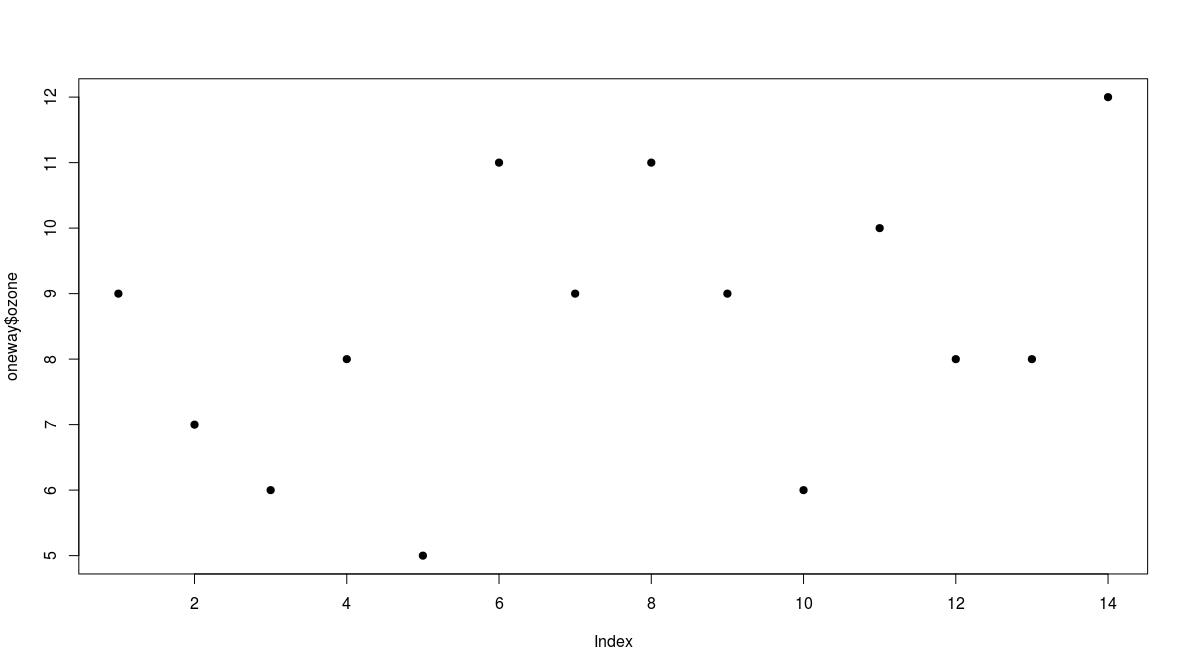
\includegraphics[width=11cm]{TSS1.png}
\end{center}
\end{frame}

\begin{frame}\frametitle{Total Sum of Squares}
  \begin{itemize}
  \item  there is a lot of scatter, indicating that the variance in ozone is large
  \item to get a feel for the overall variance we plot the overall mean (8.5) and indicate each of the residuals by a vertical line
  \end{itemize}
\end{frame}

\begin{frame}\frametitle{Total Sum of Squares}
\begin{center}
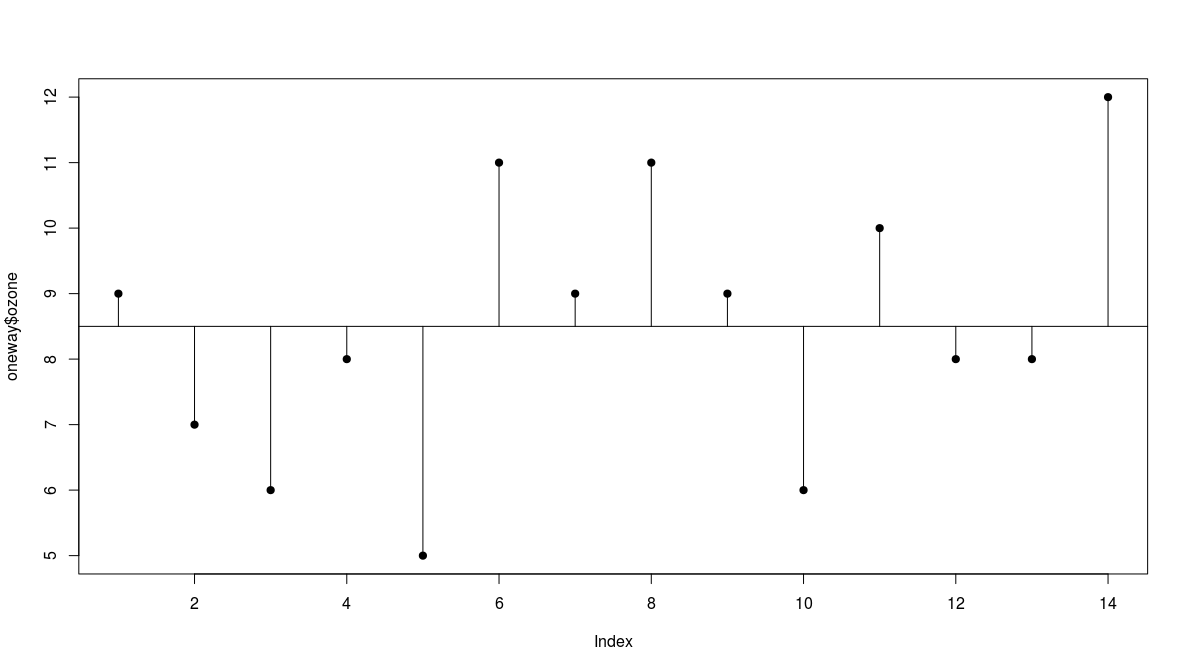
\includegraphics[width=11cm]{img/TSS.png}
\end{center}
\end{frame}

\begin{frame}\frametitle{Total Sum of Squares}
  \begin{itemize}
  \item we refer to this overall variation as the \emph{total sum of squares, SSY or TSS} 
$$ SSY = \sum(y-\bar{y})^2$$
  \end{itemize}
\end{frame}

\begin{frame}\frametitle{Total Sum of Squares}
  \begin{itemize}
  \item in this case $$SSY = 55.5$$
  \end{itemize}
   \tikzstyle{background grid}=[draw, black!50,step=.5cm]
        \begin{tikzpicture}
            % Put the graphic inside a node. This makes it easy to place the
            % graphic and to draw on top of it. 
            % The above right option is used to place the lower left corner
            % of the image at the (0,0) coordinate. 
            \node [inner sep=0pt,above right] 
                {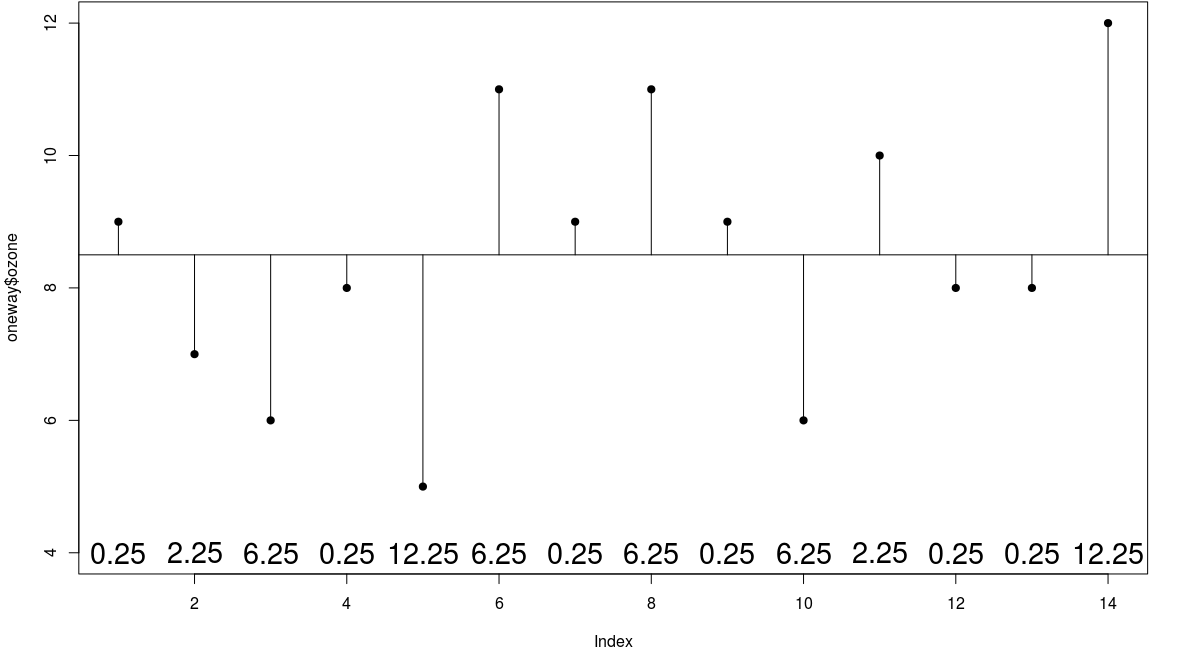
\includegraphics[width=11cm]{TSS2.png}};
            \filldraw[fill=blue!40,opacity=.5] (5.7,1.1) ellipse (5cm and 0.5cm);
%%            \fill (21.5,1.8) circle (2pt);
            % define destination coordinates
        \end{tikzpicture}
\end{frame}

\begin{frame}\frametitle{Group Means}
  \begin{itemize}
  \item now instead of fitting the overall mean, let us fit the individual garden means
  \end{itemize}
\begin{table}[ht]
\centering
\begin{tabular}{lcc}
  \hline
garden & a & b \\ 
  mean &  7 & 10 \\ 
   \hline
\end{tabular}
\end{table}
\end{frame}

\begin{frame}\frametitle{Group Means}
\tikzstyle{na} = [baseline=-.5ex]
  \begin{columns}
    \begin{column}{0.7\paperwidth}
      \begin{itemize}
      \item[]  \tikz[na] \coordinate (s-A); Garden A
      \end{itemize}
    \end{column}
    \begin{column}{0.4\paperwidth}
      \begin{itemize}
      \item[] Garden B \tikz[na] \coordinate (s-B);
      \end{itemize}
    \end{column}
  \end{columns}
%%  \tikzstyle{background grid}=[draw, black!50,step=.5cm]
        \begin{tikzpicture}
            % Put the graphic inside a node. This makes it easy to place the
            % graphic and to draw on top of it. 
            % The above right option is used to place the lower left corner
            % of the image at the (0,0) coordinate. 
            \node [inner sep=0pt,above right] 
            {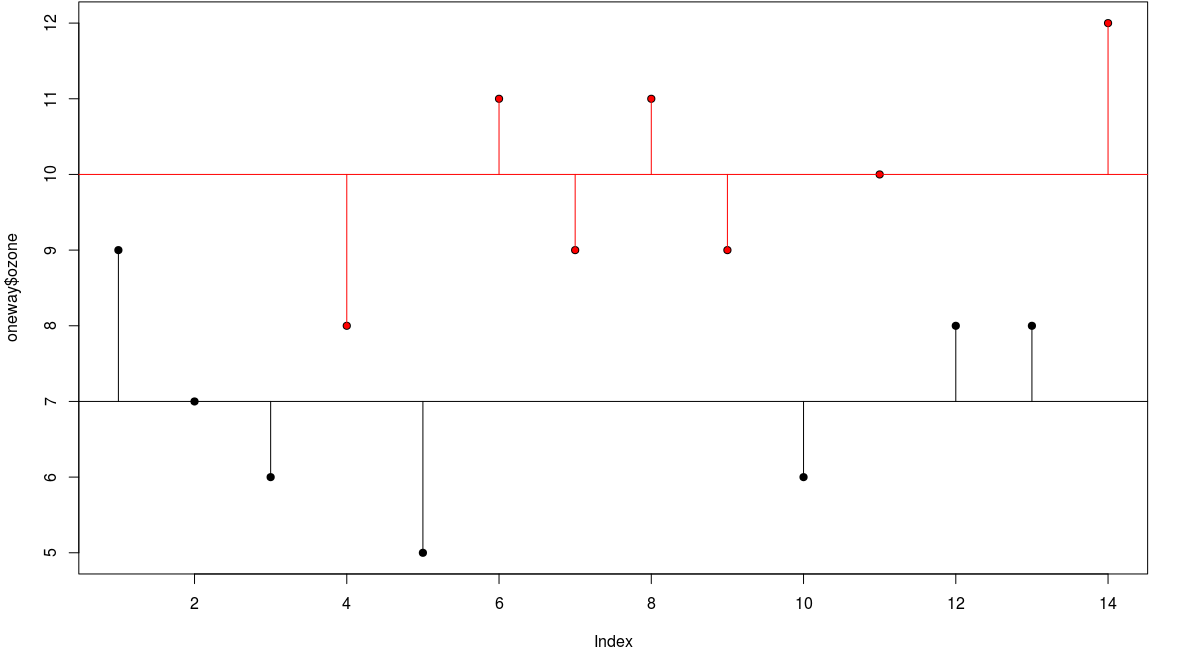
\includegraphics[width=10cm]{img/ESS.png}};
            % define destination coordinates
            \path (9.75,4.2) coordinate (B)
            (.6,2.3) coordinate (A);
        \end{tikzpicture}

% define overlays
% Note the use of the overlay option. This is required when 
% you want to access nodes in different pictures.
\begin{tikzpicture}[overlay]
        \path[->,red,thick] (s-B) edge [bend left] (B);
        \path[->,black,thick] (s-A) edge [bend right] (A);
\end{tikzpicture}

\end{frame}


\begin{frame}\frametitle{Group Means}
  \begin{itemize}
  \item now we see that the mean ozone concentration is substantially higher in garden B
  \item the aim of ANOVA is to determine 
    \begin{itemize}
    \item whether it is significantly higher \emph{or}
    \item whether this kind of difference could come by chance alone
    \end{itemize}
  \end{itemize}
\end{frame}

\begin{frame}\frametitle{Error Sum of Squares}
\emph{ When the means are significantly different then the sum of squares computed from the individual garden means will be smaller than the sum of squares computed from the overall mean. }
  \begin{itemize}
  \item we define the new sum of squares as the \emph{error sum of squares} (error in the sense of 'residual')
$$ SSE = \sum(y_{garden A}-\bar{y}_{garden A})^2+\sum(y_{garden B}-\bar{y}_{garden B})^2$$
  \end{itemize}
\end{frame}

\begin{frame}\frametitle{Total Sum of Squares}
  \begin{itemize}
  \item in this case $$SSE = 24.0$$
  \end{itemize}
\begin{center}
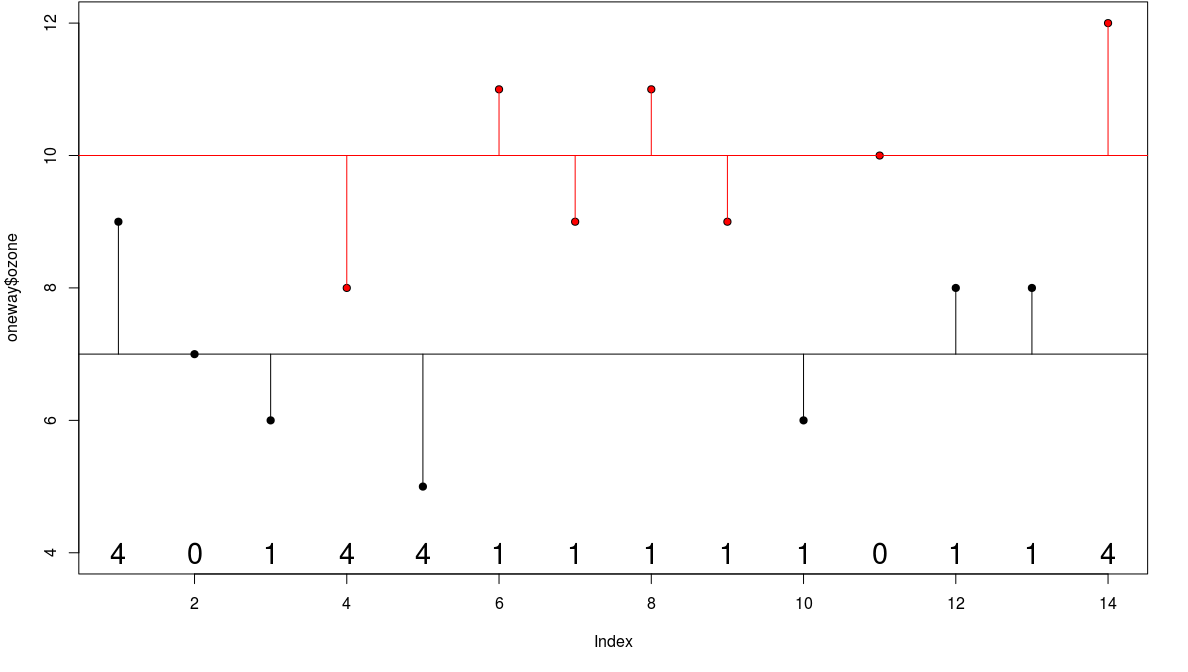
\includegraphics[width=10cm]{img/ESS2.png}
\end{center}
\end{frame}


\begin{frame}\frametitle{Treatment Sum of Squares}
\begin{itemize}
  \item then the component of the variation that is explained by the difference of the means is called the \emph{treatment sum of squares} SSA
  \item analysis of variance is based  on the notion that we break down the total sum of squares into useful and informative components
$$SSY=SSE+SSA$$ where
    \begin{itemize}
      \item SSA = explained variation
      \item SSE = unexplained variation
    \end{itemize}

  \end{itemize}
\end{frame}

\begin{frame}\frametitle{ANOVA table}
\begin{center}
\small
%% \rowcolors{1}{gray!10}{gray!30}
\begin{tabular}{@{} >{\ttfamily}l cccr}
\hline
Source & Sum of squares & Degrees of freedom & Mean square & F ratio \\
\hline
Garden &  $31.5$ & $1$ &  $31.5$ &  $15.75$\\
Error &  $24.0$ & $12$ &  $s^2=2.0$ &  \\
Total & $55.5$ & $13$ & & \\   \hline
\end{tabular}
\end{center}
\end{frame}


\begin{frame}[fragile]\frametitle{ANOVA}
  \begin{itemize}
  \item now we need to test whether an F ratio of 15.75 is large or small
  \item we can use a table or software package
  \item I use here software to calculate the cumulative probability
  \end{itemize}
\begin{verbatim}
> 1 - pf(15.75,1,12)
[1] 0.001864103
\end{verbatim}
\end{frame}

\begin{frame}\frametitle{ANOVA}
\begin{center}
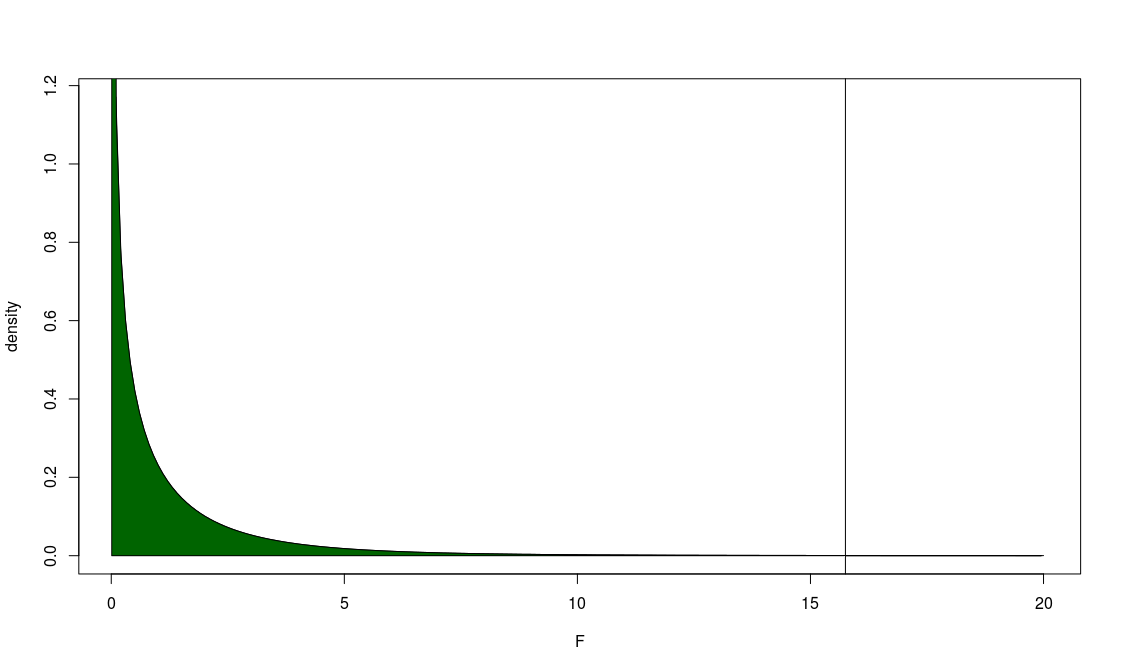
\includegraphics[width=10cm]{img/fdens.png}
\end{center}
\end{frame}


\begin{frame}[fragile]\frametitle{ANOVA in R}
  \begin{itemize}
  \item in R we use the \texttt{lm()} or the \texttt{aov()} command and
  \item the formula syntax \texttt{a \sim  b}
  \item we assign this to an variable
 \end{itemize}
\end{frame}


\begin{frame}[fragile]\frametitle{ANOVA in R}
\begin{verbatim}
mm <- lm(ozone ~ garden, data=oneway)
mm

Call:
lm(formula = ozone ~ garden, data = oneway)

Coefficients:
(Intercept)      gardenb  
          7            3  
\end{verbatim}
\end{frame}


\begin{frame}[fragile]\frametitle{ANOVA in R}
\footnotesize
\begin{verbatim}
> summary(mm)

Call:
lm(formula = ozone ~ garden, data = oneway)

Residuals:
   Min     1Q Median     3Q    Max 
    -2     -1      0      1      2 

Coefficients:
            Estimate Std. Error t value Pr(>|t|)    
(Intercept)   7.0000     0.5345  13.096 1.82e-08 ***
gardenb       3.0000     0.7559   3.969  0.00186 ** 
---
Signif. codes:  0 ‘***’ 0.001 ‘**’ 0.01 ‘*’ 0.05 ‘.’ 0.1 ‘ ’ 1

Residual standard error: 1.414 on 12 degrees of freedom
Multiple R-squared:  0.5676,	Adjusted R-squared:  0.5315 
F-statistic: 15.75 on 1 and 12 DF,  p-value: 0.001864
\end{verbatim}
\end{frame}

\begin{frame}[fragile]\frametitle{ANOVA in R}
\footnotesize
\begin{verbatim}
> anova(mm)
Analysis of Variance Table

Response: ozone
          Df Sum Sq Mean Sq F value   Pr(>F)   
garden     1   31.5    31.5   15.75 0.001864 **
Residuals 12   24.0     2.0                    
---
Signif. codes:  0 ‘***’ 0.001 ‘**’ 0.01 ‘*’ 0.05 ‘.’ 0.1 ‘ ’ 1
\end{verbatim}
\end{frame}



\begin{frame}[fragile,allowframebreaks]\frametitle{ANOVA in R}
\footnotesize
\begin{verbatim}
> m2 <- aov(ozone ~ garden, data=oneway)
> m2
Call:
   aov(formula = ozone ~ garden, data = oneway)

Terms:
                garden Residuals
Sum of Squares    31.5      24.0
Deg. of Freedom      1        12

Residual standard error: 1.414214
Estimated effects may be unbalanced
> summary(m2)
            Df Sum Sq Mean Sq F value  Pr(>F)   
garden       1   31.5    31.5   15.75 0.00186 **
Residuals   12   24.0     2.0                   
---
Signif. codes:  0 ‘***’ 0.001 ‘**’ 0.01 ‘*’ 0.05 ‘.’ 0.1 ‘ ’ 1
> summary.lm(m2)

Call:
aov(formula = ozone ~ garden, data = oneway)

Residuals:
   Min     1Q Median     3Q    Max 
    -2     -1      0      1      2 

Coefficients:
            Estimate Std. Error t value Pr(>|t|)    
(Intercept)   7.0000     0.5345  13.096 1.82e-08 ***
gardenb       3.0000     0.7559   3.969  0.00186 ** 
---
Signif. codes:  0 ‘***’ 0.001 ‘**’ 0.01 ‘*’ 0.05 ‘.’ 0.1 ‘ ’ 1

Residual standard error: 1.414 on 12 degrees of freedom
Multiple R-squared:  0.5676,	Adjusted R-squared:  0.5315 
F-statistic: 15.75 on 1 and 12 DF,  p-value: 0.001864

> summary(m2)
            Df Sum Sq Mean Sq F value  Pr(>F)   
garden       1   31.5    31.5   15.75 0.00186 **
Residuals   12   24.0     2.0                   
---
Signif. codes:  0 ‘***’ 0.001 ‘**’ 0.01 ‘*’ 0.05 ‘.’ 0.1 ‘ ’ 1
\end{verbatim}
\end{frame}



\begin{frame}\frametitle{ANOVA Assumptions}
  \begin{alertblock}{Central Assumptions}
  \begin{itemize}
  \item independed, normal distributed errors
  \item equality of variances (homogeneity)
  \end{itemize}
  \end{alertblock}
\end{frame}


\begin{frame}[allowframebreaks]\frametitle{Welch ANOVA}
\begin{itemize}
\item generalization of the Welch t-test
\item tests whether the means of the outcome variables are different across the factor levels
\item assumes sufficiently large sample (greater than 10 times the number of groups in the calculation, groups of size one are to be excluded)
\item sensitive to the existence of outliers (only few are allowed)
\item the r command is \texttt{oneway.test()}
\item non-parametric alternative \texttt{kruskal.test()}
\end{itemize}
\end{frame}


\begin{frame}\frame{Exercises}
  \begin{enumerate}
  \item Look at the help of the TukeyHSD function. What is its purpose? 
  \item Execute the code of the example near the end of the help page, interpret the results!
  \item install and load the granovaGG package (a package for visualization of ANOVAs), load the \texttt{arousal} data frame and use the \texttt{stack()} command to bring the data in the long form. Do a anova analysis. Is there a difference at least 2 of the groups? If indicated do a post-hoc test.
  \item Visualize your results
  \end{enumerate}
\end{frame}



\begin{frame}[allowframebreaks,fragile]\frametitle{Exercises - Solutions}
  \begin{enumerate}
  \item Look at the help of the TukeyHSD function. What is its purpose? 
  \item Execute the code of the example near the end of the help page, interpret the results!
  \item install and load the granovaGG package (a package for visualization of ANOVAs), load the \texttt{arousal} data frame and use the \texttt{stack()} command to bring the data in the long form. Do a anova analysis. Is there a difference at least 2 of the groups? If indicated do a post-hoc test.\scriptsize
\begin{verbatim}
> require(granovaGG)
> data(arousal)
> datalong <- stack(arousal)
> m1 <- aov(values ~ ind, data = datalong)
> summary(m1)
            Df Sum Sq Mean Sq F value   Pr(>F)    
ind          3  273.4   91.13   10.51 4.17e-05 ***
Residuals   36  312.3    8.68                     
---
Signif. codes:  0 ‘***’ 0.001 ‘**’ 0.01 ‘*’ 0.05 ‘.’ 0.1 ‘ ’ 1
> TukeyHSD(m1)
  Tukey multiple comparisons of means
    95% family-wise confidence level

Fit: aov(formula = values ~ ind, data = datalong)

$ind
                  diff           lwr        upr     p adj
Drug.A.B-Drug.A   3.54  -0.007542384  7.0875424 0.0506601
Drug.B-Drug.A    -0.45  -3.997542384  3.0975424 0.9860554
Placebo-Drug.A   -3.84  -7.387542384 -0.2924576 0.0296168
Drug.B-Drug.A.B  -3.99  -7.537542384 -0.4424576 0.0223986
Placebo-Drug.A.B -7.38 -10.927542384 -3.8324576 0.0000137
Placebo-Drug.B   -3.39  -6.937542384  0.1575424 0.0654726
\end{verbatim}\normalsize
  \item Visualize your results\scriptsize
\begin{verbatim}
> ggplot(datalong,aes(x=ind,y=values)) + 
+        geom_boxplot()  
\end{verbatim}
\begin{center}
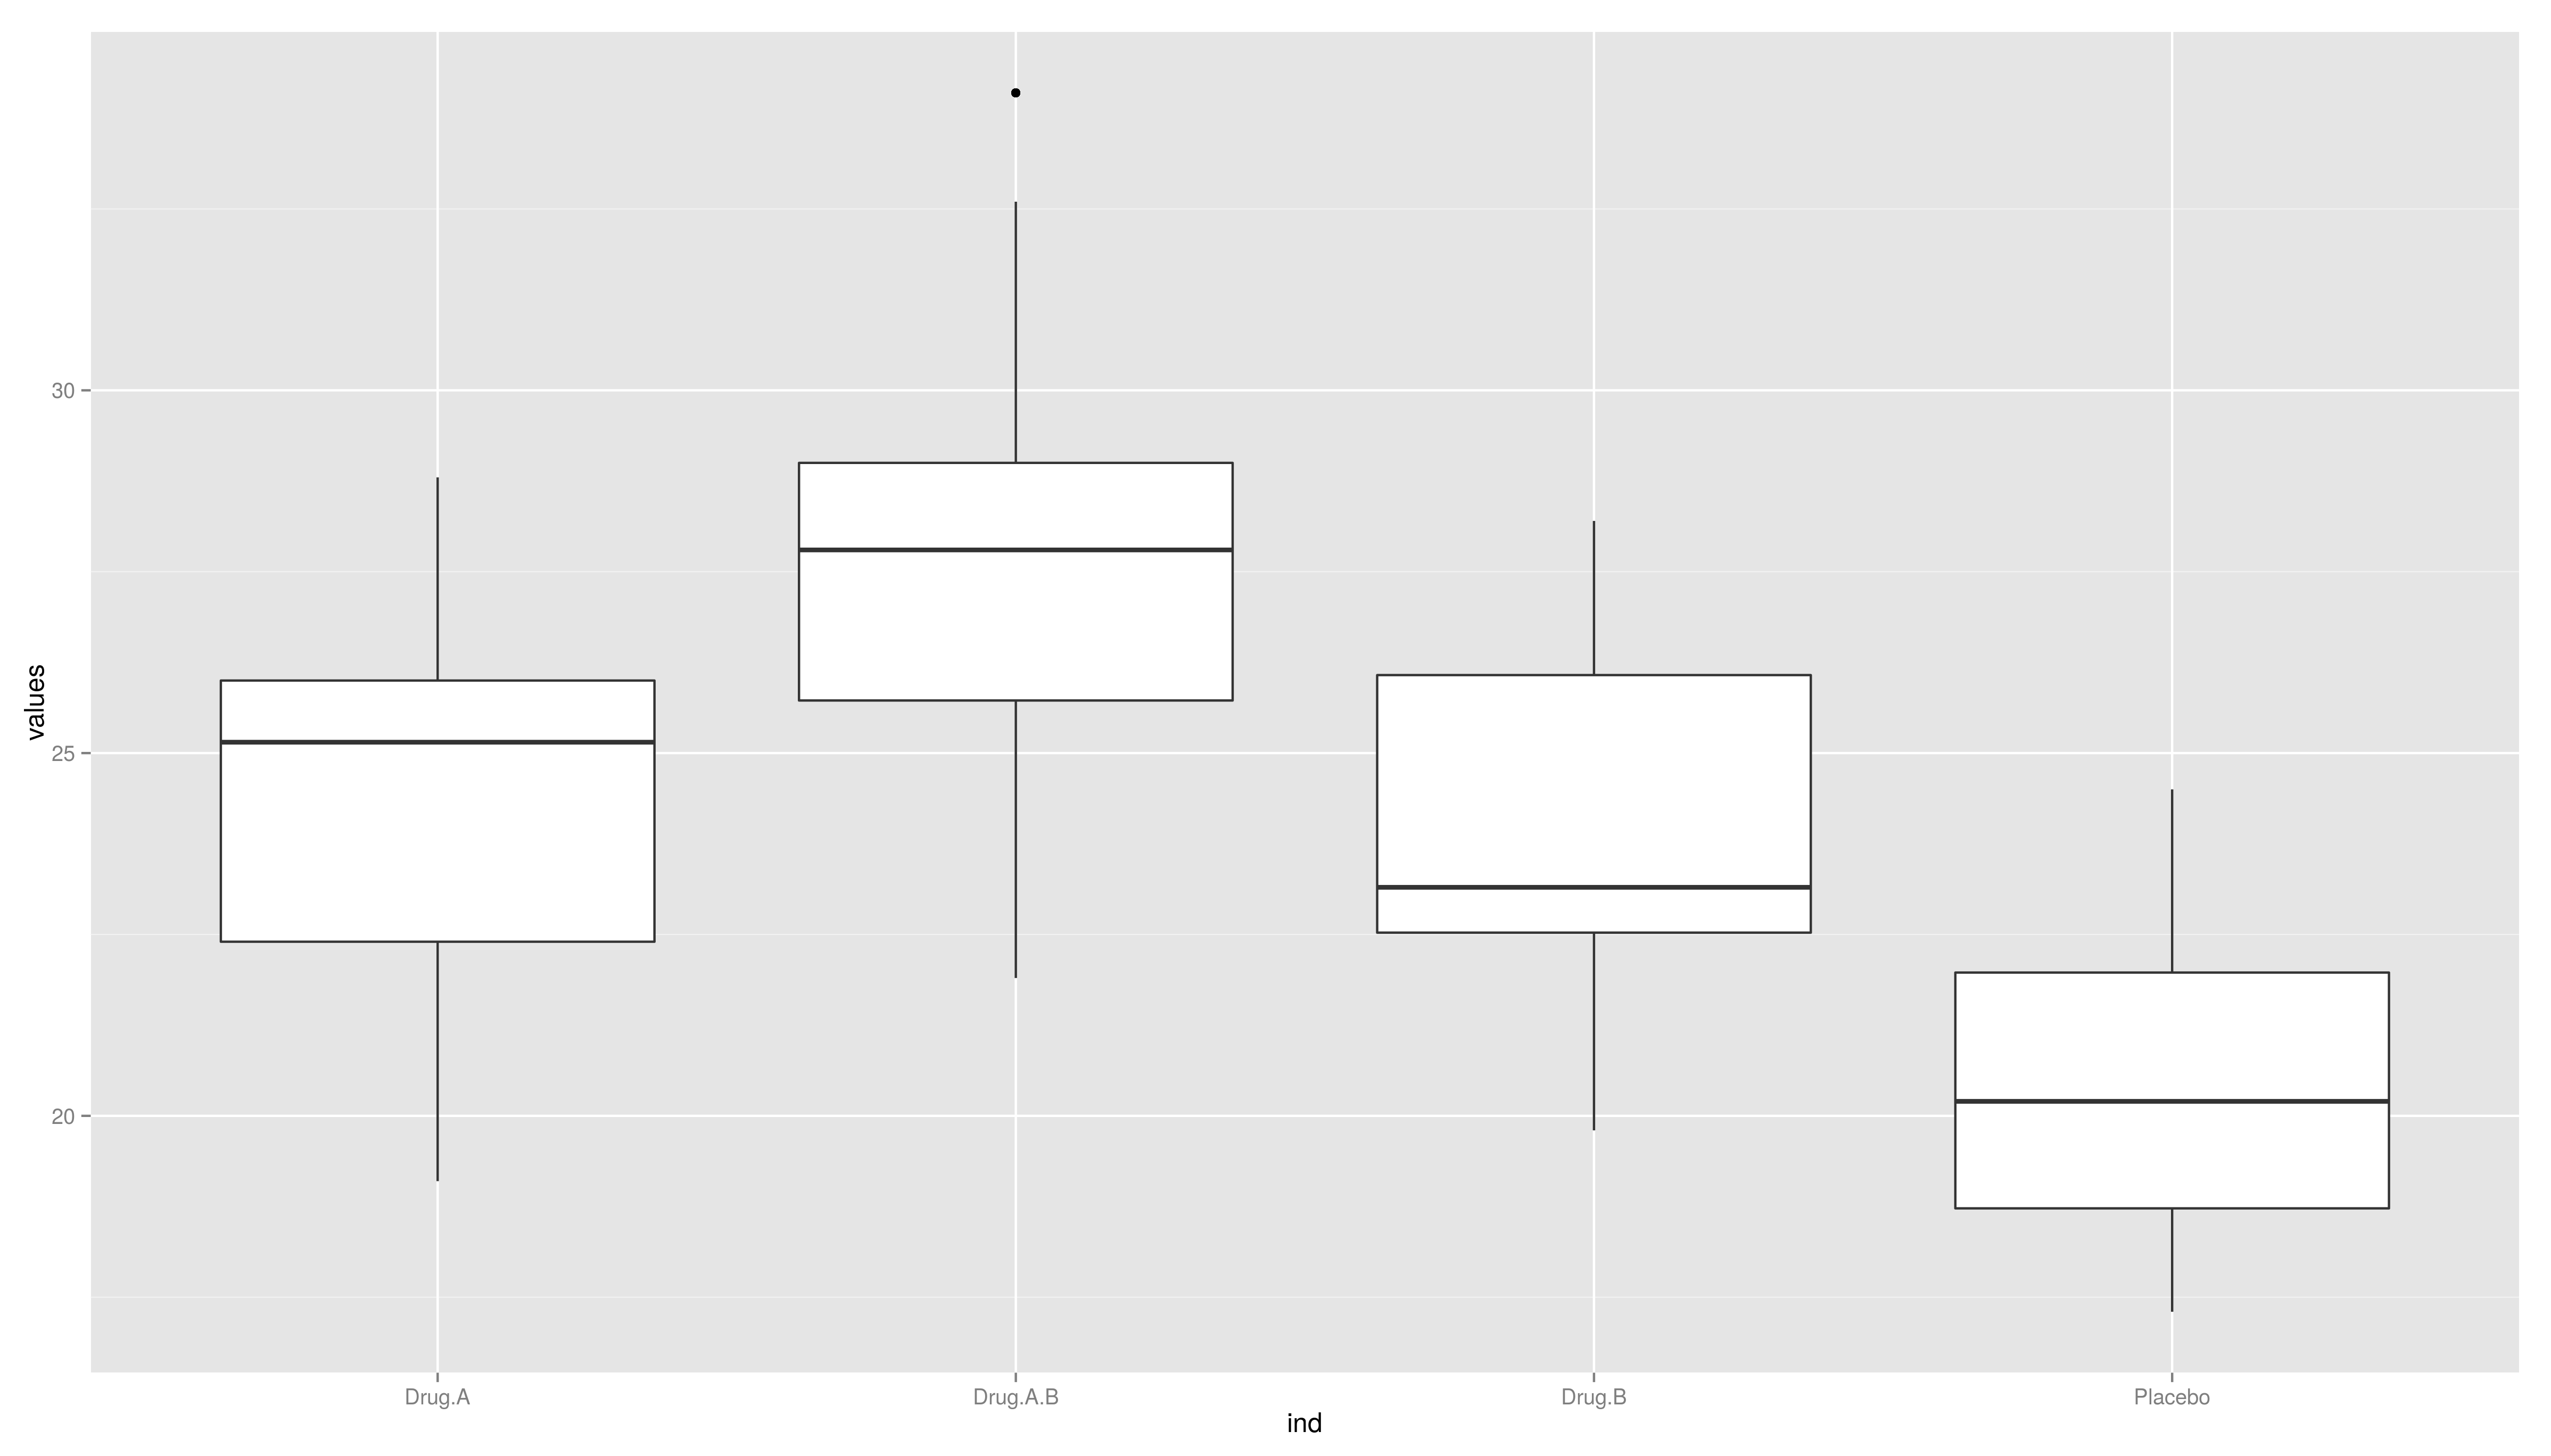
\includegraphics[width=10cm]{img/aovgr1.png}
\end{center}
\begin{verbatim}
> granovagg.1w(datalong$values,group = datalong$ind)

By-group summary statistics for your input data (ordered by group means)
     group group.mean trimmed.mean contrast variance standard.deviation
4  Placebo      20.43        20.30    -3.65     5.83               2.41
3   Drug.B      23.82        23.85    -0.26     7.50               2.74
1   Drug.A      24.27        24.45     0.19     7.89               2.81
2 Drug.A.B      27.81        27.52     3.73    13.49               3.67
  group.size
4         10
3         10
1         10
2         10

Below is a linear model summary of your input data

Call:
lm(formula = score ~ group, data = owp$data)

Residuals:
   Min     1Q Median     3Q    Max 
-5.910 -2.015 -0.075  1.885  6.290 

Coefficients:
              Estimate Std. Error t value Pr(>|t|)    
(Intercept)    24.2700     0.9314  26.057  < 2e-16 ***
groupDrug.A.B   3.5400     1.3172   2.688  0.01083 *  
groupDrug.B    -0.4500     1.3172  -0.342  0.73461    
groupPlacebo   -3.8400     1.3172  -2.915  0.00608 ** 
---
Signif. codes:  0 ‘***’ 0.001 ‘**’ 0.01 ‘*’ 0.05 ‘.’ 0.1 ‘ ’ 1

Residual standard error: 2.945 on 36 degrees of freedom
Multiple R-squared:  0.4668,	Adjusted R-squared:  0.4223 
F-statistic:  10.5 on 3 and 36 DF,  p-value: 4.173e-05

\end{verbatim}
\begin{center}
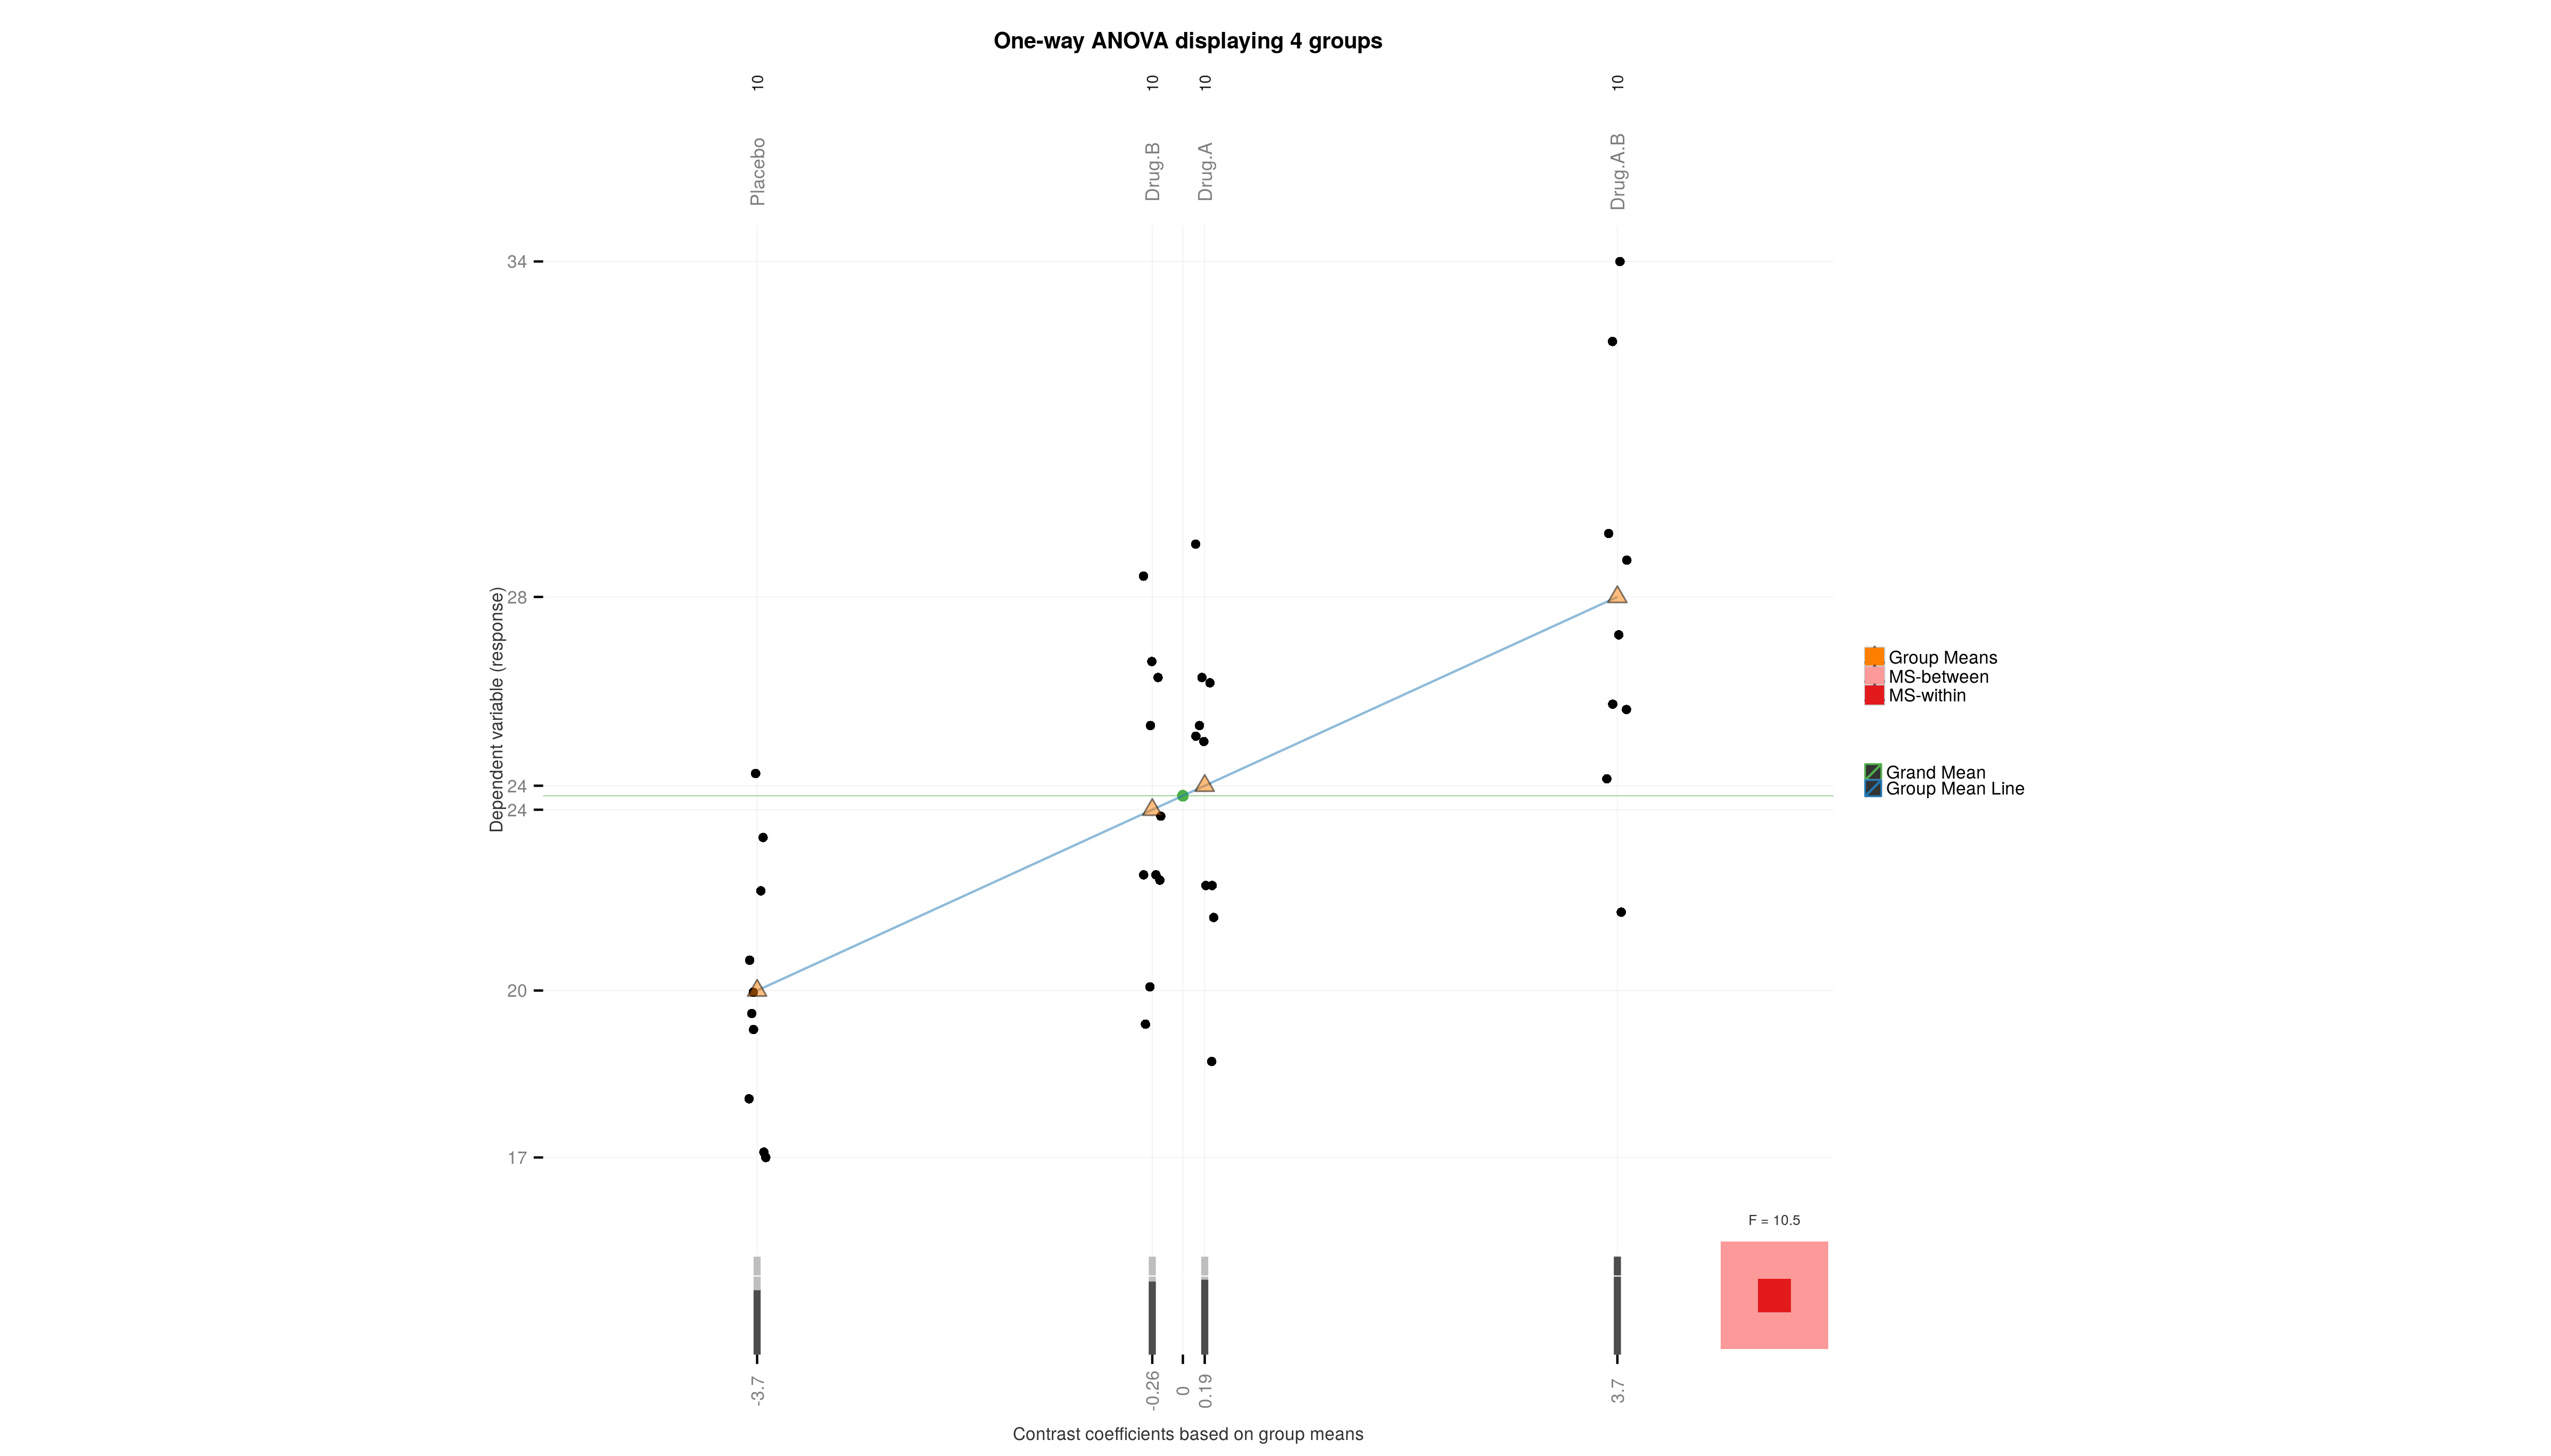
\includegraphics[width=10cm]{img/aovgr2.png}
\end{center}
  \end{enumerate}
\end{frame}




\end{document}
